\documentclass[a4paper,onecolumn,oneside,12pt,extrafontsizes]{memoir}
\usepackage[utf8]{inputenc}
\usepackage[T1]{fontenc}
\usepackage[english,polish]{babel}
\usepackage{setspace}
\usepackage{color,calc}
\usepackage{ebgaramond}
\usepackage{tgtermes}
\usepackage{float}

\renewcommand*\ttdefault{txtt}

\clubpenalty=10000
\widowpenalty=10000
\righthyphenmin=3

\renewcommand{\topfraction}{0.95}
\renewcommand{\bottomfraction}{0.95}
\renewcommand{\textfraction}{0.05}
\renewcommand{\floatpagefraction}{0.35}

\setlength{\headsep}{10pt}
\setlength{\headheight}{13.6pt}
\setlength{\footskip}{\headsep+\headheight}
\setlength{\uppermargin}{\headheight+\headsep+1cm}
\setlength{\textheight}{\paperheight-\uppermargin-\footskip-1.5cm}
\setlength{\textwidth}{\paperwidth-5cm}
\setlength{\spinemargin}{2.5cm}
\setlength{\foremargin}{2.5cm}
\setlength{\marginparsep}{2mm}
\setlength{\marginparwidth}{2.3mm}

\checkandfixthelayout[fixed]

\linespread{1}
\setlength{\parindent}{14.5pt}

\usepackage{multicol}
\usepackage{tabularx}
\usepackage{listings}
\usepackage{xpatch}
\makeatletter
\xpatchcmd\l@lstlisting{1.5em}{0em}{}{}
\makeatother

\lstset{
  basicstyle=\small\ttfamily,
  breaklines=true,
  postbreak=\mbox{\textcolor{red}{$\hookrightarrow$}\space},
  belowskip=.5\baselineskip,
  literate={\_}{{\_\allowbreak}}1
}

\definecolor{lightgray}{rgb}{.9,.9,.9}
\definecolor{darkgray}{rgb}{.4,.4,.4}
\definecolor{purple}{rgb}{0.65, 0.12, 0.82}
\definecolor{javared}{rgb}{0.6,0,0} % for strings
\definecolor{javagreen}{rgb}{0.25,0.5,0.35} % comments
\definecolor{javapurple}{rgb}{0.5,0,0.35} % keywords
\definecolor{javadocblue}{rgb}{0.25,0.35,0.75} % javadoc

\lstdefinelanguage{JavaScript}{
	keywords={typeof, new, true, false, catch, function, return, null, catch, switch, var, if, in, while, do, else, case, break},
	keywordstyle=\color{blue}\bfseries,
	ndkeywords={class, export, boolean, throw, implements, import, this},
	ndkeywordstyle=\color{darkgray}\bfseries,
	identifierstyle=\color{black},
	sensitive=false,
	comment=[l]{//},
	morecomment=[s]{/*}{*/},
	commentstyle=\color{purple}\ttfamily,
	stringstyle=\color{red}\ttfamily,
	morestring=[b]',
	morestring=[b]"
}

\lstdefinestyle{JavaScriptStyle}{
	language=JavaScript,
	commentstyle=\color{javagreen},
	backgroundcolor=,
	extendedchars=true,
	basicstyle=\footnotesize\ttfamily,
	showstringspaces=false,
	showspaces=false,
	numbers=none,%left,
	numberstyle=\footnotesize,
	numbersep=9pt,
	tabsize=2,
	breaklines=true,
	breakatwhitespace=true,
	showtabs=false,
	captionpos=t
}

\definecolor{pblue}{rgb}{0.13,0.13,1}
\definecolor{pgreen}{rgb}{0,0.5,0}
\definecolor{pred}{rgb}{0.9,0,0}
\definecolor{pgrey}{rgb}{0.46,0.45,0.48}
\definecolor{dark-grey}{rgb}{0.4,0.4,0.4}

\newcommand\JSONnumbervaluestyle{\color{blue}}
\newcommand\JSONstringvaluestyle{\color{red}}

\newif\ifcolonfoundonthisline

\makeatletter

\lstdefinestyle{json-style}
{
	showstringspaces    = false,
	keywords            = {false,true},
	alsoletter          = 0123456789.,
	morestring          = [s]{"}{"},
	stringstyle         = \ifcolonfoundonthisline\JSONstringvaluestyle\fi,
	MoreSelectCharTable =%
	\lst@DefSaveDef{`:}\colon@json{\processColon@json},
	basicstyle          = \footnotesize\ttfamily,
	keywordstyle        = \ttfamily\bfseries,
	numbers				= left,
	numberstyle={\footnotesize\ttfamily\color{dark-grey}},
	xleftmargin			= 2em
}

\newcommand\processColon@json{
	\colon@json
	\ifnum\lst@mode=\lst@Pmode
	\global\colonfoundonthislinetrue
	\fi
}

\lst@AddToHook{Output}{
	\ifcolonfoundonthisline
	\ifnum\lst@mode=\lst@Pmode
	\def\lst@thestyle{\JSONnumbervaluestyle}
	\fi
	\fi
	\lsthk@DetectKeywords
}

\lst@AddToHook{EOL}
{\global\colonfoundonthislinefalse}

\makeatother

\usepackage{memlays}
\usepackage{printlen}
\usepackage{enumitem}

\uselengthunit{pt}
\makeatletter
\newcommand{\showFontSize}{\f@size pt} % makro wypisujące wielkość bieżącej czcionki
\makeatother

\usepackage{enumitem}
\setlist{noitemsep,topsep=4pt,parsep=0pt,partopsep=4pt,leftmargin=*}
\setenumerate{labelindent=0pt,itemindent=0pt,leftmargin=!,label=\arabic*.}
\setlistdepth{4}
\setlist[itemize,1]{label=$\bullet$}
\setlist[itemize,2]{label=\normalfont\bfseries\textendash}
\setlist[itemize,3]{label=$\ast$}
\setlist[itemize,4]{label=$\cdot$}
\renewlist{itemize}{itemize}{4}

\makeatletter
\renewenvironment{quote}{
	\begin{list}{}
	{
	\setlength{\leftmargin}{1em}
	\setlength{\topsep}{0pt}%
	\setlength{\partopsep}{0pt}%
	\setlength{\parskip}{0pt}%
	\setlength{\parsep}{0pt}%
	\setlength{\itemsep}{0pt}
	}
	}{
	\end{list}}
\makeatother

\usepackage[pdftex,bookmarks,breaklinks,unicode]{hyperref}
\usepackage{hyperxmp}
\usepackage{ifpdf}

\ifpdf
 \usepackage{datetime2}
 \usepackage[pdftex]{graphicx}
 \DeclareGraphicsExtensions{.pdf,.jpg,.mps,.png}
\pdfcompresslevel=9
\pdfoutput=1

\makeatletter
\AtBeginDocument{
  \hypersetup{
	pdfinfo={
    Title = {\@title},
    Author = {\@author},
    Subject={Praca dyplomowa \ifMaster magisterska\else inżynierska\fi},
    Keywords={\@kvpl},
		Producer={},
	  CreationDate= {},
    ModDate={\pdfcreationdate},
		Creator={pdftex},
	}}
}

\pdftrailerid{}
\pdfsuppressptexinfo15
\makeatother
\else
\usepackage{graphicx}
\DeclareGraphicsExtensions{.eps,.ps,.jpg,.mps,.png}
\fi
\sloppy

\def\UrlBreaks{\do\/\do-\do_}

\setcounter{secnumdepth}{2}
\setcounter{tocdepth}{2}
\setsecnumdepth{subsection}

\makeatletter
\def\@seccntformat#1{\csname the#1\endcsname.\quad}
\def\numberline#1{\hb@xt@\@tempdima{#1\if&#1&\else.\fi\hfil}}
\makeatother

\renewcommand{\chapternumberline}[1]{#1.\quad}
\renewcommand{\cftchapterdotsep}{\cftdotsep}

\makeatletter
\renewcommand*{\insertchapterspace}{%
  \addtocontents{lof}{\protect\addvspace{3pt}}%
  \addtocontents{lot}{\protect\addvspace{3pt}}%
	\addtocontents{toc}{\protect\addvspace{3pt}} %
  \addtocontents{lol}{\protect\addvspace{3pt}}}
\makeatother

\setlength{\cftbeforechapterskip}{0pt}
\renewcommand{\aftertoctitle}{\afterchaptertitle\vspace{-4pt}}

\captionnamefont{\small}
\captiontitlefont{\small}

\newcommand{\listingcaption}[1]
{%
\vspace*{\abovecaptionskip}\small
\refstepcounter{lstlisting}\hfill%
Listing \thelstlisting: #1\hfill%\hfill%
\addcontentsline{lol}{lstlisting}{\protect\numberline{\thelstlisting}#1}
}%

\newcommand{\eng}[1]{(ang.~\emph{#1})}
\newcommand*{\captionsource}[2]{
  \caption[{#1}]{
    #1 \emph{Źródło:} #2
  }%
}

\addto\captionspolish{
\renewcommand{\tablename}{Tab.}
}

\addto\captionspolish{
\renewcommand{\figurename}{Rys.}
}

\addto\captionspolish{
\renewcommand{\lstlistlistingname}{Spis listingów}
}

\addto\captionspolish{
\renewcommand{\bibname}{Literatura}
}

\addto\captionspolish{
\renewcommand{\listfigurename}{Spis rysunków}
}

\addto\captionspolish{
\renewcommand{\listtablename}{Spis tabel}
}

\addto\captionspolish{
\renewcommand\indexname{Indeks rzeczowy}
}

\renewcommand{\abstractnamefont}{\normalfont\Large\bfseries}
\renewcommand{\abstracttextfont}{\normalfont}

\addtopsmarks{headings}{
    \nouppercaseheads
}{
\createmark{chapter}{both}{shownumber}{}{. \space}
\createmark{section}{right}{shownumber}{}{. \space}
}

\makeatletter
\copypagestyle{outer}{headings}
\makeoddhead{outer}{}{}{\small\itshape\rightmark}
\makeevenhead{outer}{\small\itshape\leftmark}{}{}
\makeoddfoot{outer}{\small\@author:~\@titleShort}{}{\small\thepage}
\makeevenfoot{outer}{\small\thepage}{}{\small\@author:~\@title}
\makeheadrule{outer}{\linewidth}{\normalrulethickness}
\makefootrule{outer}{\linewidth}{\normalrulethickness}{2pt}
\makeatother

\copypagestyle{plain}{headings}
\makeoddhead{plain}{}{}{}
\makeevenhead{plain}{}{}{}
\makeevenfoot{plain}{}{}{}
\makeoddfoot{plain}{}{}{}

\copypagestyle{empty}{headings}
\makeoddhead{empty}{}{}{}
\makeevenhead{empty}{}{}{}
\makeevenfoot{empty}{}{}{}
\makeoddfoot{empty}{}{}{}

\newif\ifMaster

\makeatletter
%Uczelnia
\newcommand\uczelnia[1]{\renewcommand\@uczelnia{#1}}
\newcommand\@uczelnia{}
%Wydział
\newcommand\wydzial[1]{\renewcommand\@wydzial{#1}}
\newcommand\@wydzial{}
%Kierunek
\newcommand\kierunek[1]{\renewcommand\@kierunek{#1}}
\newcommand\@kierunek{}
%Specjalność
\newcommand\specjalnosc[1]{\renewcommand\@specjalnosc{#1}}
\newcommand\@specjalnosc{}
%Tytuł po angielsku
\newcommand\titleEN[1]{\renewcommand\@titleEN{#1}}
\newcommand\@titleEN{}
%Tytuł krótki
\newcommand\titleShort[1]{\renewcommand\@titleShort{#1}}
\newcommand\@titleShort{}
%Promotor
\newcommand\promotor[1]{\renewcommand\@promotor{#1}}
\newcommand\@promotor{}
%Słowa kluczowe
\newcommand\kvpl[1]{\renewcommand\@kvpl{#1}}
\newcommand\@kvpl{}
\newcommand\kven[1]{\renewcommand\@kven{#1}}
\newcommand\@kven{}
%Komenda wykorzystywana w streszczeniu
\newcommand\mykeywords{\hspace{\absleftindent}%
\parbox{\linewidth-2.0\absleftindent}{
       \iflanguage{polish}{\textbf{Słowa kluczowe:} \@kvpl}{%
			 \iflanguage{english}{\textbf{Keywords:} \@kven}}{}}
				}

\def\maketitle{
  \pagestyle{empty}
    \fontfamily{\ebgaramond@family}\selectfont

\newlength{\tmpfboxrule}
\setlength{\tmpfboxrule}{\fboxrule}
\setlength{\fboxsep}{2mm}
\setlength{\fboxrule}{0mm}

\setlength{\unitlength}{1mm}
\begin{picture}(0,0)

\put(20,-124){\fbox{
\parbox[c][71mm][c]{104mm}{\centering
{\fontsize{18pt}{20pt}\bfseries\selectfont \@title}\\[5mm]
{\fontsize{18pt}{20pt}\bfseries\selectfont \@titleEN}\\[10mm]
{\fontsize{16pt}{18pt}\selectfont \@author}}
}
}
\end{picture}
\setlength{\fboxrule}{\tmpfboxrule}
{\vskip 9pt\centering
		{\fontsize{20pt}{22pt}\bfseries\selectfont \@uczelnia}\\[5pt]
		{\fontsize{16pt}{18pt}\bfseries\selectfont \@wydzial}\\[1pt]
		  \hrule
	}
{\vskip 24pt\raggedright\fontsize{14pt}{16pt}\selectfont%
\begin{tabular}{@{}ll}
Kierunek: & {\bfseries \@kierunek}\\
Specjalność: & {\bfseries \@specjalnosc}\\
\end{tabular}\\[1.3cm]
}
{\vskip 29pt\centering{\fontsize{24pt}{26pt}\selectfont%
{\fontsize{26pt}{28pt}\selectfont P}RACA {\fontsize{26pt}{24pt}\selectfont D}YPLOMOWA\\[7pt]
\ifMaster \selectfont{\fontsize{26pt}{28pt}\selectfont M}AGISTERSKA\\[2.5cm]%
\else \selectfont{\fontsize{26pt}{28pt}\selectfont I}NŻYNIERSKA\\[2.5cm]\fi
}}
	\vfill
{\centering
    {\fontsize{14pt}{16pt}\selectfont Opiekun pracy}\\[2mm]
	{\fontsize{14pt}{16pt}\bfseries\selectfont \@promotor}\\[10mm]
}
\vspace{4cm}\noindent
{\fontsize{12pt}{14pt}\selectfont Słowa kluczowe: \@kvpl}
\vspace{1.3cm}
\hrule\vspace*{0.3cm}
{\centering
{\fontsize{14pt}{16pt}\selectfont \@date}\\[0cm]
}
\normalfont
 \cleardoublepage
}
\makeatother

\title{Aplikacja webowa do optymalizacji zleceń w transporcie towarów} % INFO: tytuł pracy w języku polskim
\titleShort{Aplikacja webowa do optymalizacji zleceń w transporcie towarów}  % INFO: krótki tytuł pracy (do zamieszczenia w stopce, sklejony z imieniem i nazwiskiem autora nie powinien zająć więcej niż jedną linijkę)
\titleEN{Web application for optimizing orders in the transport of goods} % INFO: tytuł pracy w języku angielskim
\author{Krystian Tomczyk}  % INFO: imię i nazwisko autora
\uczelnia{Politechnika Wrocławska} % INFO: nazwa uczelni
\wydzial{Wydział Informatyki i Telekomunikacji} % INFO: nazwa wydziału
\kierunek{Informatyka techniczna (ITE)} % IFO: nazwa kierunku
\specjalnosc{Inżynieria systemów informatycznych (INS)} % INFO: nazwa specjalności
\promotor{dr. inż. Paweł Rogaliński} % INFO: dane promotora
\kvpl{aplikacja, transport, web} % INFO: słowa kluczowe po polsku
\kven{application, transport, web} % INFO: słowa kluczowe po angielsku
\date{WROCŁAW, 2024} % INFO: miejscowość, rok złożenia pracy dyplomowej

\begin{document}

\pdfbookmark[0]{Tytuł}{Tytul.1}
\maketitle

\pdfbookmark[0]{Streszczenie}{streszczenie.1}
\begin{abstract}
Niniejsza praca inżynierska dotyczy projektu aplikacji webowej CargoLink, zaprojektowanej w celu optymalizacji procesów logistycznych w transporcie towarów. Głównym celem systemu jest łączenie zleceniodawców i przewoźników, minimalizowanie pustych przebiegów oraz redukcja kosztów transportu. Aplikacja oferuje funkcje takie jak: dodawanie zleceń transportowych, publikowanie ogłoszeń o planowanych trasach, rekomendacje dopasowanych ofert oraz komunikację użytkowników poprzez wbudowany czat. System wspiera generowanie szablonów umów oraz umożliwia ocenę użytkowników po zakończeniu współpracy.

Pod względem technicznym aplikacja wykorzystuje nowoczesne technologie, takie jak TypeScript, Next.js, Tailwind CSS i PostgreSQL, zapewniające wysoką wydajność i bezpieczeństwo. W bazie danych zastosowano UUID jako klucze główne oraz algorytm bcrypt do szyfrowania haseł. Interfejs użytkownika zaprojektowano w programie Figma z uwzględnieniem responsywności oraz intuicyjnej obsługi.

Dokumentacja opisuje szczegółowo przypadki użycia systemu dla różnych aktorów oraz architekturę warstwową aplikacji. Przedstawiono również proces testowania systemu, w tym testy jednostkowe, end-to-end oraz wydajnościowe. Na zakończenie wskazano potencjalne kierunki rozwoju projektu, takie jak wprowadzenie nowych funkcjonalności i zwiększenie skalowalności systemu.
\end{abstract}
\mykeywords
{
\selectlanguage{english}
\begin{abstract}
This engineering thesis concerns the design of CargoLink web application, developed to optimize logistics processes in cargo transportation. The main goal of the system is to connect shippers with carriers, minimize empty runs, and reduce transportation costs. The application offers features such as: adding transport orders, publishing announcements about planned routes, recommending matched offers, and enabling user communication through a built-in chat. The system supports generating contract templates and allows users to rate each other after completed cooperation.

From a technical perspective, the application utilizes modern technologies such as TypeScript, Next.js, Tailwind CSS, and PostgreSQL, ensuring high performance and security. The database implements UUID as primary keys and uses the bcrypt algorithm for password encryption. The user interface was designed in Figma with consideration for responsiveness and intuitive operation.

The documentation thoroughly describes use cases for various actors and the layered architecture of the application. The system testing process is also presented, including unit tests, end-to-end tests, and performance tests. Finally, potential directions for project development are indicated, such as introducing new functionalities and increasing system scalability.
\end{abstract}
\mykeywords
}

\pagestyle{outer}
\clearpage

\pdfbookmark[0]{Spis treści}{spisTresci.1}
\tableofcontents*
\clearpage

\pdfbookmark[0]{Spis rysunków}{spisRysunkow.1}
\listoffigures*
\clearpage

% \pdfbookmark[0]{Spis tabel}{spisTabel.1}
% \listoftables*
% \clearpage

% \pdfbookmark[0]{Spis listingów}{spisListingow.1}
% \lstlistoflistings*
% \clearpage

\chapterstyle{default}
\chapter{Wstęp}

Transport towarów odgrywa kluczową rolę w globalnej gospodarce, łącząc producentów i konsumentów na całym świecie. Efektywność transportu ma bezpośredni wpływ na koszty operacyjne firm oraz na ceny finalnych produktów \cite{MurphyWoodLogistyka}. W zależności od specyfiki przewożonych towarów oraz potrzeb zleceniodawców, transport może przyjmować dwie następujące formy:

\label{sec:przewoz_regularny}
Transport regularny, inaczej łańcuch dostaw, to przewóz towarów, który odbywa się według ustalonego harmonogramu i stałych tras. Charakteryzuje się regularnością kursów, co oznacza, że pojazdy wykonują swoje trasy w określonych, z góry ustalonych terminach. Przykładami transportu regularnego są linie autobusowe, kolejowe czy lotnicze, które działają według stałego rozkładu jazdy.

\label{sec:transport_okazjonalny}
Transport okazjonalny to przewóz towarów, który odbywa się bez ustalonego z góry rozkładu jazdy. Pojazdy wykonują swoje trasy w zależności od zapotrzebowania klientów, najczęściej jest to usługa jednorazowa. Sam przewóz zaś zlecany jest na potrzebę klienta, nie musi on jednak określać dokładnego terminu odbycia trasy, ani przez kogo ma on być zrealizowany.

Podczas swoich tras przewoźnicy czasami są zmuszeni do przebycia części drogi bez żadnego ładunku. Powoduje to, że przewozy nie są w pełni zoptymalizowane względem kosztów, jakie niesie za sobą pokonywana trasa. Możliwe jest jednak zredukowanie występowania takich sytuacji poprzez odpowiednie powiązanie przewoźników i osób zlecających transport okazjonalny. Zleceniodawca, który nie potrzebuje dostawy towaru w konkretnej dacie, mógłby wtedy zlecić transport z nieokreślonym dokładnie terminem dotarcia towaru, w zamian za niższe ceny przewozowe. Przykład: dyrektor szkoły, w czasie wakacji, zamówił dużych rozmiarów tablicę interaktywną, która nie zmieściłaby się w standardowym samochodzie osobowym. Z racji, że zamówienie zostało złożone w czasie, gdy dzieci nie chodzą do szkoły, nie zależy mu na dokładnym terminie dostawy. Może on w takim przypadku zlecić dostawę tablicy w formie transportu okazjonalnego, z mniejszymi kosztami transportu. Przewoźnik mógłby zabrać towar i zawieźć go na miejsce docelowe, gdy akurat wykonywałby trasę bez ładunku i kierował się w przybliżonym kierunku. Taka sytuacja jest korzystna dla obu stron, przewoźnik może odbywać przewozy bardziej efektywnie, dzięki nie marnowaniu zasobów na puste przebiegi. Zleceniodawca natomiast, może oczekiwać niższych kosztów przewozu towarów.

Połączenie między osobami zlecającymi usługi transportowe - zleceniodawcami, a osobami oferującymi przewóz towaru - przewoźnikami, może odbywać się za pomocą serwisu oferującego dodawanie publicznych ogłoszeń. Ogłoszenia dzielić się będą na dwie kategorie, ogłoszenie z planowaną trasą przejazdu oraz zlecenie z wymaganym towarem do przewiezienia z punktu początkowego do punktu docelowego.

\section{Cel i zakres projektu}
\label{sec:cele}
Celem projektu jest stworzenie aplikacji webowej, pod tytułem \texttt{CargoLink}. Serwis ten pozwalać będzie na dodawanie ogłoszeń oraz zleceń dotyczących transportów okazjonalnych. Aplikacja przyczni się do zoptymalizowania procesów logistycznych, eliminując nieefektywne wykorzystanie zasobów transportowych. Dodatkowo pozwoli ona przewoźnikom i zleceniodawcom, na łatwą i szybką komunikacje między sobą.
Główne cele projektu:
\begin{enumerate}
    \item \textbf{Możliwość umieszczania ogłoszeń i zleceń}: aplikacja pozwalać ma na dodawanie ogłoszeń o trasach przejazdu, planowanych przez przewoźników oraz zleceń transportowych na konkretny towar przez zleceniodawców
    \item \textbf{Ułatwienie szukania odpowiednich ogłoszeń i zleceń}: poprzez system powiązania zleceń transportowych do planowanych tras przewoźników oraz ogłoszeń o planowanej trasie do zleceń zamieszczonych w serwisie, aplikacja skróci czas potrzebny na znalezienie odpowiednich ofert.
    \item \textbf{Komunikacja między przewoźnikami i zleceniodawcami}: aplikacja umożliwi szybką komunikację między użytkownikami serwisu poprzez czat tekstowy.
    \item \textbf{Redukcja kosztów transportu}: dzięki lepszemu dopasowaniu potencjalnych przewoźników i zleceniodawców, aplikacja pozwoli na obniżenie kosztów transportu zarówno dla zleceniodawców, jak i przewoźników.
\end{enumerate}
Nowoczesna aplikacja transportowa powinna przyczynić się do efektywnego zrealizowania tych celów, co wspomoże rynek zleceń transportowych, przynosząc korzyści zarówno dla zleceniodawców, jak i przewoźników.

\section{Wymagania aplikacji}
Na podstawie analizy celów wymienionych w podrozdziale \ref{sec:cele}, można wywnioskować, że do efektywnego działania serwisu, będą musiały zostać zrealizowane następujące wymagania funkcjonalne:
\begin{enumerate}
    \item \textbf{Uwierzytelnianie}: aplikacja będzie wykorzystywała system rejestracji oraz logowania.
    \item \textbf{Regulanim}: podczas rejestrowania się do serwisu, użytkownik musi zaakceptować regulamin korzystania z aplikacji.
    \item \textbf{Dodawanie zleceń transportowych}: serwis pomagał będzie znaleźć odpowiedniego przewoźnika poprzez udostępnienie możliwości dodania ogłoszenia zlecenia. W ogłoszeniu zlecenia znajdować się będzie:
    \begin{itemize}
        \item tytułu zlecenia,
        \item opis zlecenia (niewymagane),
        \item wymagana trasa przewozu (miejsce startu oraz miejsce docelowe),
        \item przybliżony termin dostarczenia (przedział dat),
        \item waga towarów do przewiezenia,
        \item wymiary przewożonych dóbr,
        \item kategoria każdego z towarów,
        \item informacja o wymaganych specjalnych warunkach podczas transportu (np. jedzenie wymagać będzie przewozu w odpowiedniej temperaturze, pole niewymagane),
        \item imienia i nazwiska zleceniodawcy bądź nazwy firmy, która zleceniodawca reprezentuje,
    \end{itemize}
    \item \textbf{Dodawanie ogłoszeń o planowanej trasie}: system powinien pozwalać przewoźnikom, na dodawanie publicznych informacji o planowanych przez siebie trasach. Ogłoszenie będzie składało się z:
    \begin{itemize}
        \item tytułu ogłoszenia,
        \item opisu ogłoszenia (niewymagane),
        \item planowanej trasy przewozu (miejsce startu oraz miejsce docelowe),
        \item daty planowanego przejazdu,
        \item dostępnego miejsca w pojeździe (wymiary liczone w europaletach),
        \item maksymalnej wagi towaru,
        \item marki i modelu pojazdu,
        \item danych kontaktowych,
        \item imienia i nazwiska przewoźnika bądź nazwy firmy, która przewoźnik reprezentuje,
    \end{itemize}
    \item \textbf{System rekomendacji ogłoszeń}: podczas wprowadzania danych o trasie, użytkownik będzie informowany o sugerowanych zleceniach dodanych przez innych użytkowników (np. gdy zlecenie dotyczy trasy, która w przybliżeniu pokrywa się z tą jaką przewoźnik planuje się poruszać). Analogicznie gdy zleceniodawca zamierza dodać ogłoszenie zlecenia, zostanie on poimformowany o proponowanych ogłoszeniach przewoźników.
    \item \textbf{Umożliwienie konaktu między użytkownikami}: aby zapewnnić kontakt między użytkownikami, w aplikacji zostanie dodany czat tekstowy umożliwiający korespondencje między zleceniodawcami, a przewoźnikami, bezpośrednio w aplikacji. Ma on pełnić rolę komunikacji na wzór tej  oferowanej przez tradycyjną poczte elektroniczną.
    \item \textbf{Generowanie szablonu umowy}: przewoźnik i zleceniodawca, po negocjacji warunków umowy, otrzymają wygenerowany przez serwis szablon dokumentu finalizujący transakcje.
    \item \textbf{Weryfikacja dodawanych ogłoszeń}: zanim ogłoszenie wyświetlać się będzie dla wszystkich użytkowników, moderator serwisu będzię musiał je zatwierdzić.
    \item \textbf{Graficzne przedstawienie trasy}: podczas dodawania ogłoszenia o planowanej trasie, przewoźnikowi wyświetlać się będzie mapa z zaznaczonymi trasami, dodanymi przez zleceniodawców, które przebiegają w przybliżonym kierunku. Zleceniodawcy natomiast, podczas dodawania oferty, będą widzieć mapę ze wszystkimi trasami planowanymi przez przewoźników.
    \item \textbf{System ocen użytkownika}: po 2 dniach po upływie terminu przewozu, użytkownicy będą mogli dodać opinie na temat użytkownika, którego umowa dotyczyła. Opinia składała się będzie z oceny w skali 1-5 oraz komentarza. Opinie będą wyświetlały się na stronie porfilu tego użytkownika oraz na dodanych przez niego ogłoszeniach.
\end{enumerate}
Aplikacja musi być niezawodna i przyjazna do użytkowania dla wszystkich. Do komfortowego korzystania z serwisu przez użytkowników, niezbędna będzie realizacja następujących wymagań niefunkcjonalnych
\begin{enumerate}
    \item \textbf{Innowacyjność}: Aplikacja musi używać nowoczesnych technologii, takich jak \texttt{TypeScript}, \texttt{Next.js}, \texttt{Tailwind CSS}, \texttt{Node.js} oraz bazę danych \texttt{PostgreSQL}, zapewni to wysoką wydajność, skalowalność i bezpieczeństwo aplikacji.
    \item \textbf{Intuicyjny interfejs użytkownika}: Aplikacja musi posiadać prosty i intuicyjny interfejs użytkownika, który umożliwi łatwą obsługę zarówno dla zleceniodawców, jak i przewoźników.
    \item \textbf{Dostępność na różnych urządzeniach}: Aplikacja musi responsywna i dostosowana do różnych urządzeń, takich jak komputery, tablety i smartfony, co zapewni wygodę użytkowania w dowolnym miejscu i czasie.
    \item \textbf{Wielojęzyczność}: użytkownicy korzystający z aplikacji, muszą mieć możliwość wyboru jednego z trzech przewidzianych języków: polski, angielski oraz niemiecki. Dodatkowo użytkownicy podczas rejestracji muszą mieć możliwość wybrania dowolnych języków, którymi się posługują. Informacje te będą zamieszczone na profilu użytkownika.
\end{enumerate}

\chapter{Wstęp}

\section{Cel projektu}
Celem projektu jest stworzenie aplikacji webowej do zleceń dla transportów okazjonalnych, która zoptymalizuje procesy logistyczne i wyeliminuje nieefektywne wykorzystanie zasobów transportowych. Aplikacja umożliwi użytkownikom łatwe i szybkie znalezienie odpowiedniego przewoźnika lub zleceniodawcy, co spowoduje redukcje pustych przebiegów i tym samym kosztów transportu.
Główne cele projektu:
\begin{enumerate}[labelwidth=\widthof{\ref{last-item}},label=\arabic*.]
\item Optymalizacja procesów logistycznych: Poprzez automatyzację procesu wyszukiwania i dopasowywania zleceń transportowych, aplikacja usprawni komunikację między zleceniodawcami a przewoźnikami, skracając czas potrzebny na znalezienie odpowiedniego transportu.
\item Eliminacja pustych przebiegów: Aplikacja umożliwi przewoźnikom znalezienie ładunków na trasach powrotnych, co zmniejszy liczbę pustych przebiegów i przyczyni się do oszczędności paliwa, co zredukuje koszty.
\item Redukcja kosztów transportu: Dzięki lepszemu dopasowaniu potencjalnych kontrahentów dla usług transportowych, aplikacja pozwoli na obniżenie kosztów transportu zarówno dla zleceniodawców, jak i przewoźników.
\item Poprawa bezpieczeństwa i jakości usług: Aplikacja umożliwi weryfikację kwalifikacji przewoźników oraz ocenę jakości świadczonych usług, co przyczyni się do zwiększenia bezpieczeństwa i zadowolenia klientów.
\item Ułatwienie dostępu do rynku transportowego: Aplikacja stworzy platformę, która ułatwi zarówno doświadczonym przewoźnikom, jak i nowym podmiotom na rynku. \label{last-item}
\end{enumerate}

Realizacja tych celów przyczyni się do stworzenia nowoczesnej i efektywnej aplikacji, która wspomoże rynek zleceń transportowych, przynosząc korzyści zarówno dla zleceniodawców, jak i przewoźników.

\section{Transport okazjonalny}
Transport okazjonalny to przewóz towarów, który nie spełnia definicji przewozu regularnego. Oznacza to, że odbywa się on bez ustalonego z góry rozkładu jazdy i może dotyczyć zarówno tras krajowych, jak i międzynarodowych.
Charakteryzuje się on:
\begin{itemize}
\item Brakiem stałego rozkładu jazdy. Pojazdy wykonują swoje trasy w zależności od zapotrzebowania klientów.
\item Jest inicjowany przez zleceniodawce. Przewóz zlecany jest na potrzebę klienta, nie określna on jednak, dokładnego terminu odbycia trasy.
\end{itemize}

\section{Wymagania niefunkcjonalne}
\begin{enumerate}[labelwidth=\widthof{\ref{last-item}},label=\arabic*.]
\item Innowacyjność: Wykorzystanie nowoczesnych technologii, takich jak \texttt{TypeScript}, \texttt{Next.js}, \texttt{Tailwind CSS}, \texttt{Node.js} oraz \texttt{PostgreSQL}, zapewni wysoką wydajność, skalowalność i bezpieczeństwo aplikacji.
\item Intuicyjny interfejs użytkownika: Aplikacja będzie posiadać prosty i intuicyjny interfejs użytkownika, który umożliwi łatwą obsługę zarówno dla zleceniodawców, jak i przewoźników.
\item Dostępność na różnych urządzeniach: Aplikacja będzie responsywna i dostosowana do różnych urządzeń, takich jak komputery, tablety i smartfony, co zapewni wygodę użytkowania w dowolnym miejscu i czasie.
\item Wielojęzyczność: Użytkownicy korzystający z aplikacji, będą mieli możliwość wyboru jednego z trzech przewidzianych języków: polski, angielski oraz niemiecki. Co przełoży się na międzynarodowy aspekt aplikacji.
\end{enumerate}

\section{Przypadki użycia}
\begin{figure}[ht]
	\centering
		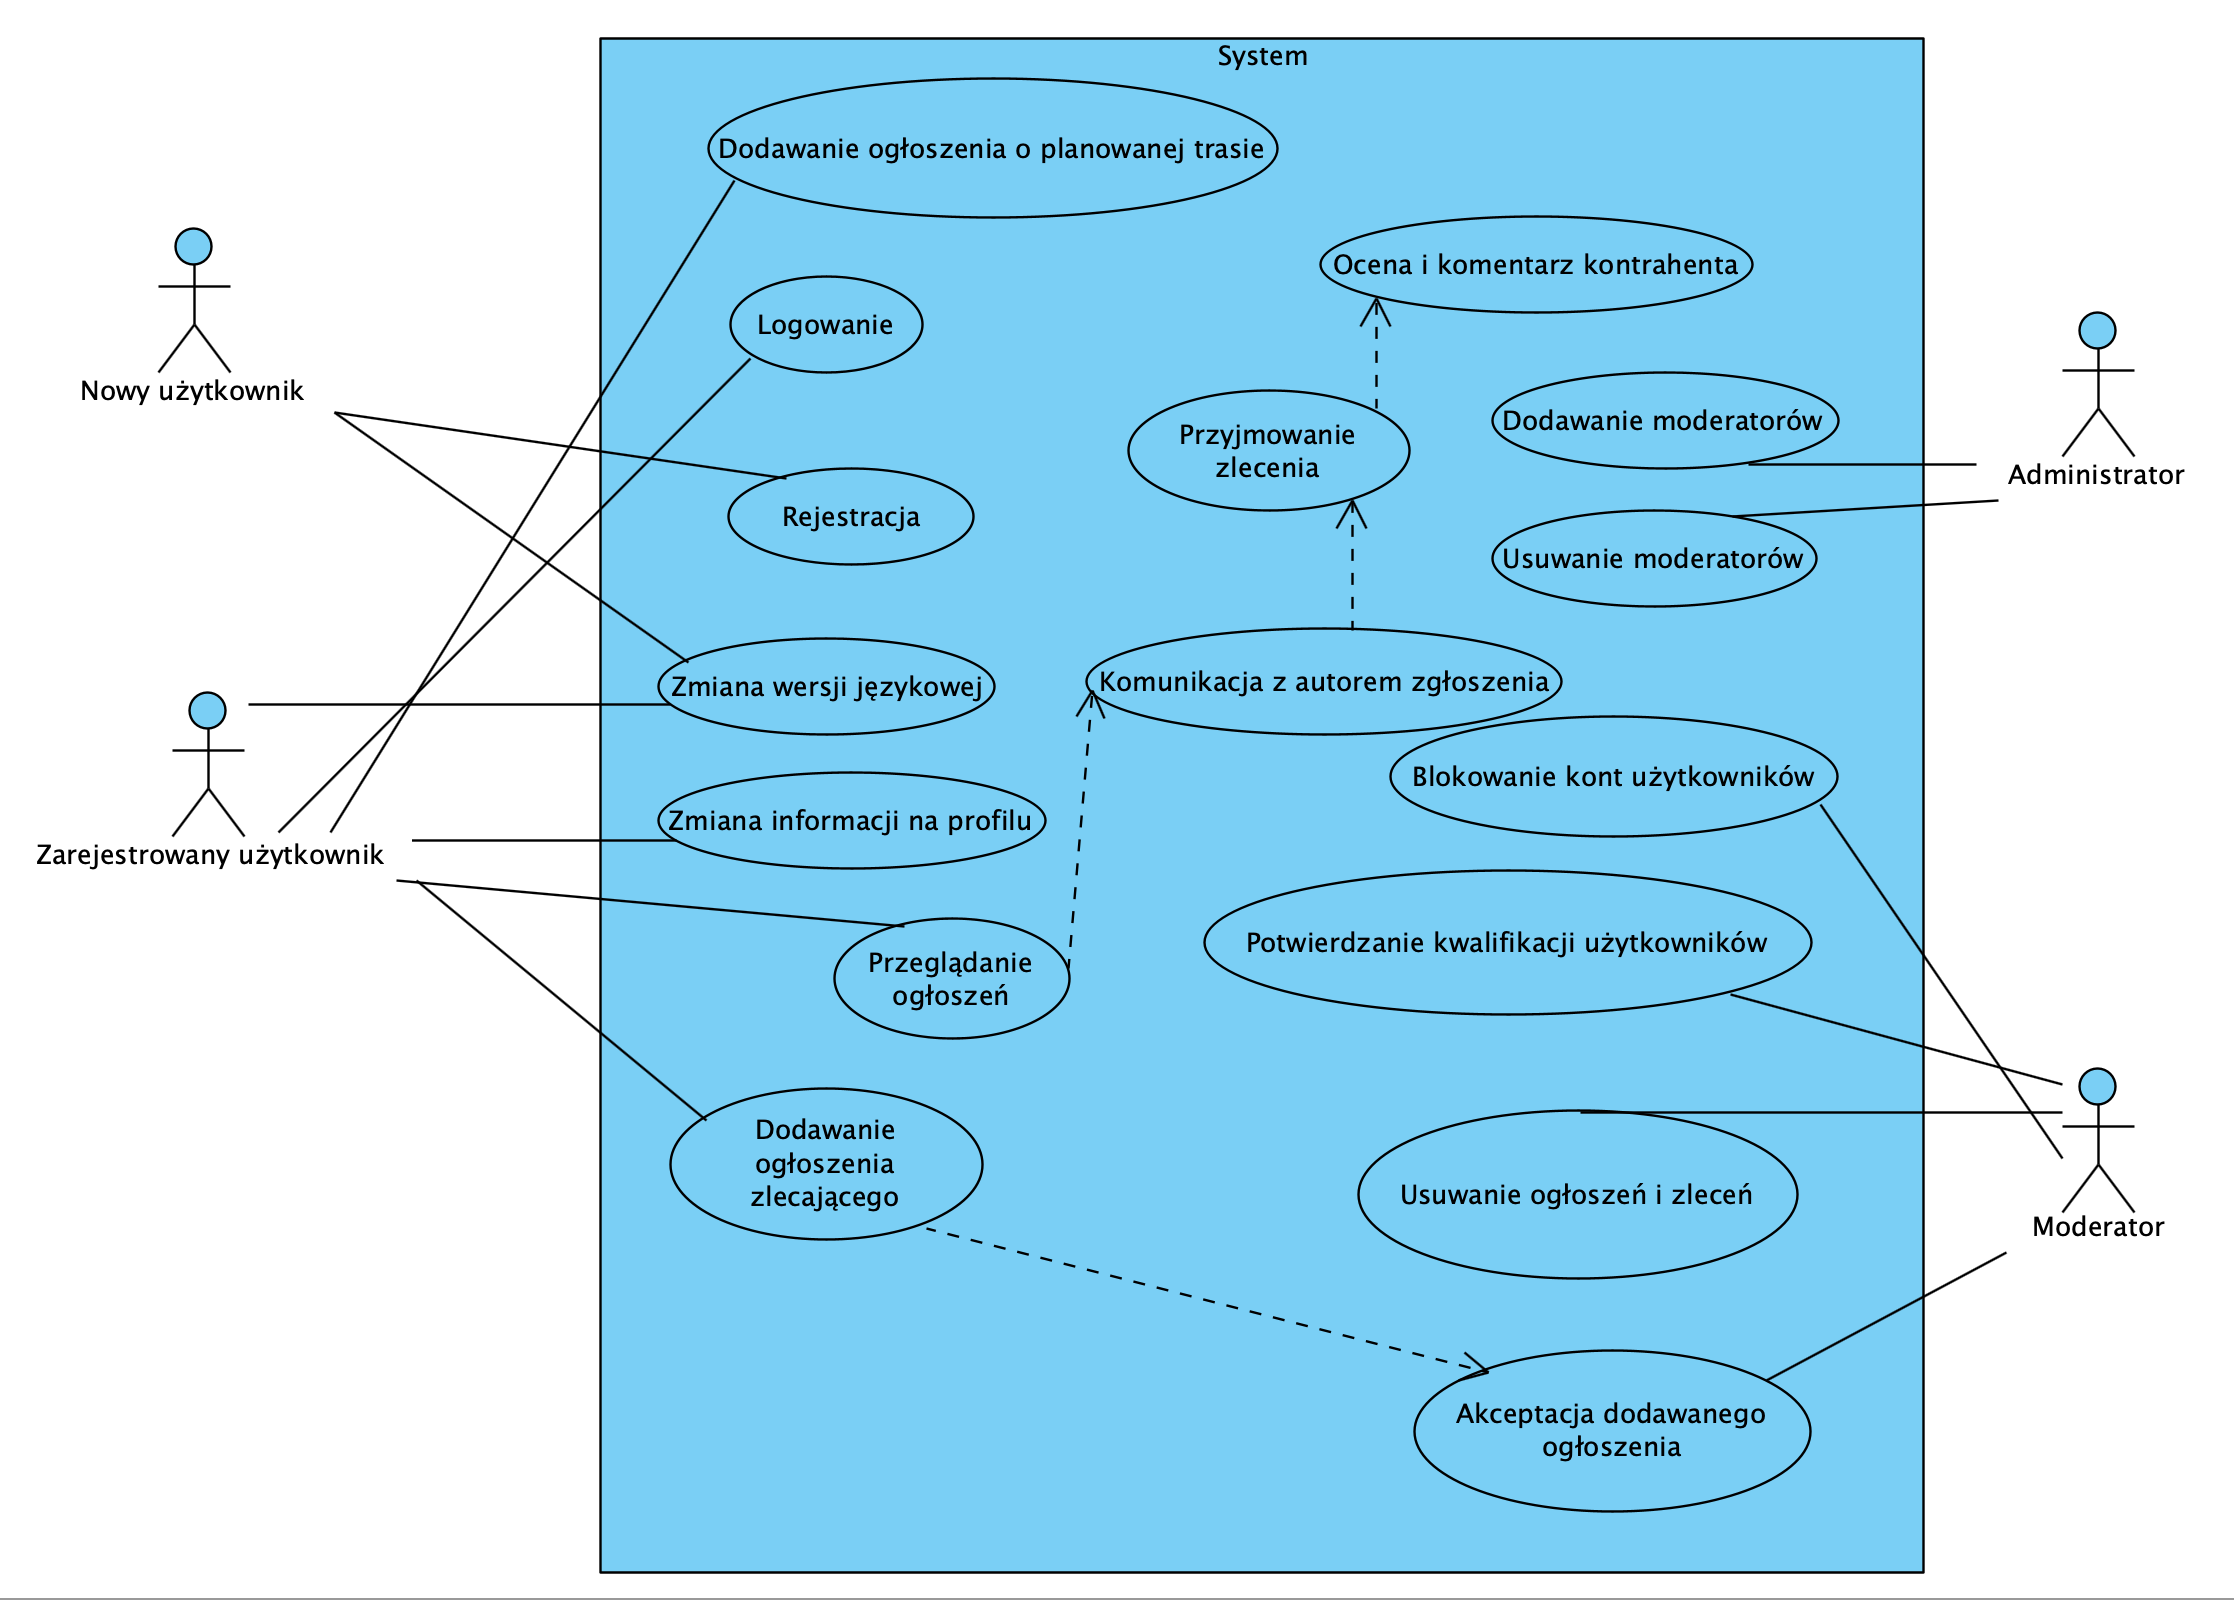
\includegraphics[width=0.9\linewidth]{rozdzial1/use_case.png}
	\caption{Przedstawienie przypadków użycia}
	\label{fig:Przedstawienie przypadków użycia}
\end{figure}


\bibliographystyle{plabbrv}
\setlength{\bibitemsep}{2pt}
\addtocontents{toc}{\addvspace{2pt}}
\bibliography{bibliografia}
\appendix

\chapter{Instrukcja wdrożeniowa}
Aplikacja jest konteneryzowana przy użyciu Docker, co zapewnia kompatybilność międzyplatformową. Baza danych jest hostowana na darmowym serwerze \texttt{Neon}, co upraszcza konfigurację.
\begin{itemize}
    \item Zainstalowane oprogramowanie \texttt{Docker}
    \item Dostęp do internetu
    \item Uprawnienia administratora
\end{itemize}
W celu wdrożenia aplikacji na środowisko produkcyjne należy wykonać następujące kroki:
\begin{enumerate}
    \item Sklonować repozytorium z GitHub.
    \item Otworzyć terminal w katalogu projektu.
    \item Zbudować obraz aplikacji za pomocą komendy \texttt{docker build -t cargolink .}.
    \item Uruchomić kontener z aplikacją za pomocą komendy \texttt{docker run -p 80:3000 cargolink}.
\end{enumerate}

Po wykonaniu powyższych kroków aplikacja będzie dostępna pod adresem \texttt{http://localhost:80}. Port na którym działa aplikacja można zmienić w pliku \texttt{Dockerfile} w linii 4. Jednak port 80 jest domyślnym portem dla protokołu HTTP, więc zaleca się pozostawienie go bez zmian. Jeżeli serwer, na którym wykonane zostały powyższe kroki, jest dostępny z zewnątrz, aplikacja będzie dostępna pod adresem \texttt{http://<adres\_serwera>:80}.

\end{document}
